\documentclass[12pt]{scrreprt}
\usepackage[utf8]{inputenc}
\usepackage[ngerman]{babel}
\usepackage[utf8]{inputenc}
\usepackage[T1]{fontenc}
\usepackage{hyperref}

%\hypersetup{colorlinks=true, citecolor=red}


\usepackage{natbib}
\usepackage[numbib]{tocbibind}
\usepackage{float}
\linespread{1.3}
\usepackage{natbib}
\usepackage{graphicx}
\usepackage{pdfpages}
\usepackage[euler]{textgreek}
\usepackage{adjustbox}
\usepackage[margin = 3cm]{geometry}


\usepackage{eso-pic} 
\usepackage{lipsum} 

\usepackage{tabularx} 
\usepackage{multirow}
\usepackage{amssymb}
\usepackage[flushleft]{threeparttable}
\usepackage{booktabs,caption}
\usepackage{color, colortbl}


\usepackage{amsmath}
\usepackage{bbm}
\usepackage{bbold}



\pagenumbering{roman}

\begin{document}
	
	\pagestyle{myheadings}

\chapter{Methodik}
In diesem Kapitel wird als erstes die Theorie hinter den Modellen erklärt. Danach gehen wir auf die Schwierigkeiten ein, denen wir gegenüberstanden. Im letzten Teil stellen wir, dann die Ergebnisse vor.
\section{Theorie}
In folgendem Kapitel soll in einem Modell der Zusammenhang einer beobachteten abhängigen Variable, in unserem Fall, der Anteil der Skitourengänger mit LVS-Gerät, durch mehrere unabhängige Variablen erklärt werden.
Für das bessere Verständis bauen wir den Theorie-Teil von einem einfachen Modell bis hin zu dem von uns verwendeten Modell auf.
\subsection{Lineares Regressionsmodell}
Bei einem linearen Regressionsmodell wird der Erwartungswert einer Zielvariable durch die Linearkombination von Einflussgrö"sen, auch Kovariablen genannt, beschrieben. Das lineare Regressionsmodell nimmt dabei folgende Form an:
\begin{align}
y_{i}= \beta_{0}+\beta_{1}x_{i1}+...+\beta_{k}x_{ik}+\epsilon_{i}
\end{align}
Die Zielgrö"se wird durch $y_{i}$ abgebildet, welche im Fall des linearen Regressionsmodells normalverteilt ist. Die Kovariablen werden durch $x_{i1},...,x_{ik}$ gekennzeichnet und $\epsilon_{i}$ stellt den Störterm dar. In Anwendungen bei denen es sich nicht um eine normalverteilte Zielvariable handelt ist das lineare Regressionsmodell unzureichend. Um das Problem zu lösen, wird im nächsten Kapitel auf das generalisierte lineare Regressionsmodell eingegangen. (Quelle: Fahrmeir S.62)
\subsection{Generalisierte lineare Regressionsmodell}
Das generalisierte lineare Regressionsmodell eignet sich für die Modellierung von Zielvariablen die nicht unbedingt normalverteilt sind. Die abhängige Variable nimmt typischerweise eine Verteilung aus einer Exponentialfamilie (z.B. Binomial, Poisson, Multinomial, Normal,...) an. In unserem Fall handelt es sich um eine durch 0 und 1 kodierte Zielvariable $y_{i}$. Die beobachtete Zielgrö"se, der Anteil an Personen mit LVS-Gerät, ist Binomial-verteilt mit $y_{i}|x_{i}\sim B(1,\pi_{i})$: \\
\begin{align}
%\vspace{0.1cm}
y_{i}=\begin{cases}
1 & \text{,wenn Person mit LVS-Gerät identifiziert wird } \\
0 & \text{,wenn Person ohne LVS-Gerät identifiziert wird.} \\
\end{cases}
\end{align}
Bei der generalisierten Regression mit binärer Zielvariable wird der Effekt der Kovariablen durch die (bedingte) Wahrscheinlichkeit $\pi_{i}$ beschrieben.
\begin{align}
\pi_{i}=P(y_{i}=1|x_{i1},...,x_{ik})=E(y_{i}|x_{i1},...,x_{ik})
\end{align}
Für den Erwartungswert der Zielvariable gilt:
\begin{align}
E(y_{i})=\pi_{i}=\frac{exp(\eta_{i})}{1+exp(\eta_{i})}=h(\eta_{i}).
\end{align}
Der Erwartungswert der Zielvariable wird mit dem linearen Prädiktor $\eta_{i}$ mittels der Responsefunktion $\pi_{i}=h(\eta_{i})$ verknüpft. Die Logit-Linkfunktion $g$ ist die Umkehrung der Responsefunktion, daher gilt:
\begin{align}
g(\pi_{i})=\log(\frac{\pi_{i}}{1-\pi_{i}}).
\end{align}
In unserer Arbeit machen wir Gebrauch von dem Logit-Link. Diese Transformation ist zur mathematischen Berechnung unseres Modells notwendig. In Kapitel (...) werden wir den Logit-Link zurücktransformieren um die Interpretation der Ergebnisse zu vereinfachen.
Das generalisierte lineare Regressionsmodell beschreibt lineare Einflüsse der Kovariablen auf die Zielvariable. In praktischen Anwendungen ist dies oft unzureichend, da neben den linearen Einflüssen auch nicht-lineare, flexible Einflüsse von Kovariablen auf die abhängige Variable wirken können (Quelle: Fahrmeir S.190). Daher wird im nächsten Kapitel die additive Regression näher erläutert.
\subsection{Additives Regressionsmodell}
Das additive Modell stellt in der Statistik ein semi-parametrisches Regressionsmodell dar. Neben mehreren nicht-linearen flexiblen Einflüssen können hier auch lineare Einflüsse von Kovariablen auf die abhängige Variable modelliert werden. \\
Das Standardmodell der additiven Regression hat die Form:
\begin{align}
y_{i}=\underbrace{\beta_{0}+\beta_{1}x_{i1}+...+\beta_{k}x_{ik}}_{\text{parametrische Effekte}}+ \underbrace{f_{1}(z_{i1})+...+f_{q}(z_{iq})}_{\text{semi-parametrische Effekte}}+\epsilon_{i}
\end{align}
Der parametrische Teil des Standardmodells hat die gleiche Form, wie schon im linearen Modell aufgezeigt. Die Funktionen $f_{1}(z_{1}),...,f_{q}(z_{q})$ werden mit nichtparametrischen Effekten geschätzt. (Quelle: Fahrmeir S.47)
Auf die Theorie hinter der Funktion $f$ wird im nächsten Kapitel eingegangen.
\subsection{Splines}
Die Schätzfunktion $f$ wird durch sogenannte Splines modelliert. Splines stellen bestimmte Funktionen dar, die stückweise aus Polynomen eines bestimmten Grades zusammengesetzt werden. Es gibt verschiedene Arten von Splines. In unserer Arbeit beschränken wir uns auf die Penalisierten Splines, die Zyklische Splines und die Thin-Plate Splines.
\subsubsection{Polynom-Splines}
	Eine Möglichkeit, die Funktion $f$ abzubilden, sind Splines, die über Polynome modelliert werden und Polynom-Splines, oder auch Regressions-Splines, genannt werden. Das polynomiale Modell hat die Form: 
\begin{align}
f(z)=\gamma_{0}+\gamma_{1}z+...+\gamma_{l}z^l,
\end{align}
wobei das Polynom vom Grad $l$ durch den Einfluss von $z$ auf $y$ modelliert wird und $\gamma_{j}$ die Regressionskoeffizienten darstellen. Um eine flexible Schätzfunktion gewährleisten zu können, wird der Definitionsbereich von $z$ in Intervalle geteilt und Polynome werden für das jeweilige Intervall geschätzt. Die Zerlegung von $z$ erfolgt stückweise auf Basis von sogenannten Knotenmengen $k_{1}$ bis $k_{m}$.  Ein Problem, welches dabei entstehen könnte ist, dass an den Intervallgrenzen keine $glatte$ Funktion entstehen. Der Graph einer $glatten$ Funktion hat an den Intervallgrenzen keine \glqq{Ecken\grqq}. Deshalb muss für die \glqq{mathematische}\grqq ~Glattheit die zusätzliche Bedingung, dass die Funktion $f(z)$ an den Intervallgrenzen $(l-1)$-mal stetig differenzierbar ist, eingeführt werden. Der Grad des Splines und die Anzahl der Knoten können somit im hohen Ma"se die Funktion beeinflussen, je höher die Anzahl an Knoten ist, desto $rauer$ ist die Funktion $f(z)$. Um Polynom-Splines in der Praxis anwenden zu können, bedarf es einer Darstellung der Menge der Polynom-Splines. Eine mögliche Darstellung eines Polynom-Splines stellt die B-Spline-Basisfunktion dar.
\subsubsection{Basis Splines}
Der B-Spline dient als Basisfunktion für Polynom-Splines. Jedoch wird sich auch der Penalisierungs-Spline, welcher im darauffolgenen Kapitel vorgestellt wird, die B-Spline-Basisfunktion zu Nutzen machen. Das Ziel bei der Konstruktion der B-Spline-Basisfunktion ist es die Polynomstücke des gewünschten Grades an den Knoten ausreichend $glatt$ zusammenzusetzen. Die Basisfunktion besteht dabei aus $(l+1)$ Polynomstücken vom Grad $l$, welche stetig an den Knoten zusammengesetzt werden. Die Funktion $f(z)$ lässt sich durch die Linearkombination der Basisfunktionen:
\begin{align}
f(z)=\sum_{j=1}^d\gamma_{j}B_{j}(z)
\end{align}
darstellen. Die Koeffizienten  $\gamma_{j}$ werden mit Hilfe der KQ-Methode geschätzt und dienen zur Skalierung der Basisfunktionen. Die Anzahl der erforderlichen Basisfunktionen $d = m+l-1$, setzt sich aus der Zahl der Knoten $m$ und den Polynomstücken des gewünschten Grades $l$, welche $(l-1)$-mal stetig differenzierbar an den Knoten aneinandergefügt werden, zusammen.  \\
Für B-Splines vom Grad 0 folgt:
\begin{align}
B_{j}^0(z)= \mathbb{1}_{[k_{j},k_{j+1}]}(z)= 
\begin{cases}
1 & k_{j} \leq z<k_{j+1};\enspace mit\enspace j=1,...,d-1; \\
0 & \text{sonst.} \\
\end{cases}
\end{align}
Für B-Splines höheren Grades gilt:
\begin{align}
B_{j}^l(z)= \frac{z-k_{j}}{k_{j+l}-k_{j}}B_{j}^{l-1}(z)+
\frac{k_{j+l+1}-z}{k_{j+l+1}-k_j+1}B_{j+1}^{l-1}(z).
\end{align}
Die Abbildung \ref{pic:b_spline} visualisiert die Schätzung eines B-Splines anhand eines fiktiven Datenbeispiels schematisch. Abbildung (a) demonstriert eine B-Spline Basis vom dritten Grad. In Abbildung (b) wird die Basisfunktion mit dem Kleinste-Quadrate-Schätzer $\hat\gamma_{j}$ skaliert. Die Abbildung (c), zeigt die erhaltene Schätzung, wenn die skalierten Basisfunktionen addiert werden.
\begin{figure}[H]
	\centering
	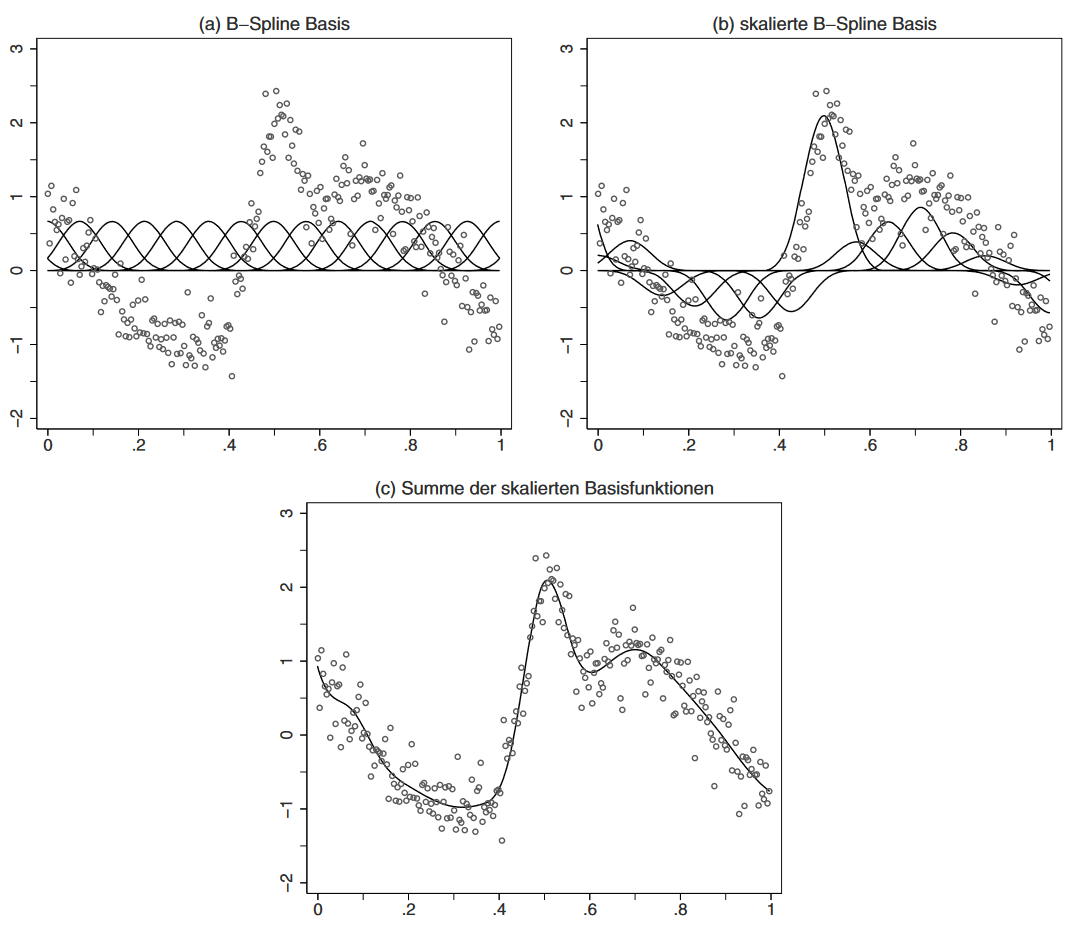
\includegraphics[width=.9\textwidth]{plots/b_spline.png}
	\caption{Schematische Darstellung der Schätzung eines nichtparametrischen Effekts mit B-Splines}
	\label{pic:b_spline}
\end{figure}

\noindent Das nächste Kapitel behandelt P-Splines, welche auf B-Splines basieren und durch einen Strafterm erweitert worden sind. In unserer Arbeit beschränken wir uns auf P-Splines.
\subsubsection{Penalisierte Splines basierend auf B-Splines}
Im vorherigen Kapitel, haben wir die Wichtigkeit der Knotenmenge kennengelernt. Die Glattheit und Flexibilität der Schätzfunktion $f(z)$ hängt stark von der Anzahl der Knoten ab. Das Ziel ist es die Funktion $f(z)$ auf Basis einer B-Spline Funktion, mit einer großen Zahl an Knoten, zu approximieren um so die Flexibilität der Schätzfunktion sicherzustellen und andererseits zu hohe Variabilität in Form eines Strafterms zu sanktionieren. Der Penalisierte-Spline, gekürzt P-Spline, kombiniert somit eine B-Spline-Basis mit einem Strafterm. Der Strafterm für B-Splines wird häufig durch die quadrierte zweite Ableitung der Schätzfunktion $f(z)$ modelliert, da diese Form im R-Paket $mgcv$ von Simon Woods implementiert wird. Die zweite Ableitung stellt ein Ma"s für die Krümmung der Funktion dar und ist daher in der Lage die Glattheit einer Funktion einzuschätzen.
Der Strafterm: 
\begin{align}
\lambda\int(f''(z))^2dz.
\end{align}
In der Anwendung wird für die Approximation der zweiten Ableitungen, die zweite Differenz des Paramters $\gamma_{j}$ verwendet. Wenn der Glättungsparameter $\lambda$ gegen unendlich konvergiert, erhält man eine nahezu lineare Schätzfunktion $f(z)$ und der Strafterm wird primär durch $\lambda$ reguliert. Im Fall von $\lambda \to 0$ verfügt der Glättungsparameter ($\lambda$) nur über ein geringers Gewicht.
\subsubsection{Zyklische P-Splines}
Eine Glättungsfunktion hei"st zyklisch, wenn die Funktion dieselben Werte und ersten Ableitungen an ihrer oberen und unteren Grenze aufweist. Beispielsweise kann man die Funktion für die Variable Woche mit Hilfe des zyklischen P-Splines modellieren. Das Ziel dabei ist es z.B den Sonntag mit dem darauffolgenden Montag zu verknüpfen. Dadurch wird sichergestellt, dass die Werte am Ende einer Woche zusammenhängend zu den Werten am Anfang der darauffolgenden Woche sind. 
Die Schätzfunktion eines zyklischen P-Splines hat die Form:
\begin{align}
f(z)=\sum_{j=1}^{k-1}B_{j}(z)\beta_{j}.
\end{align}
Der Koeffizient $\beta_{j}$ wird durch den transponierten Vektor $\beta^T=(\beta_{1},...,\beta_{k-1})$ dargestellt, wobei $\beta_{j}=\beta_{k}$ gilt.
Der Penalisierungsansatz für zyklische P-Splines ist simultan zu der Penalisierung von P-Splines basierend auf B-Splines. (Quelle: Woods S.203)
\subsubsection{Thin-Plate Splines}
Bisher wurden Funktionen mit nur einer einzigen Kovariable geschätzt. Die Thin-Plate Splines ermöglichen die Schätzung einer Funktion mit mehreren Kovariablen. In unserem Fall handelt es sich um eine Funktion mit zwei Variablen, nämlich dem Datum und der Uhrzeit. Die beiden Variablen wurden in einer Funktion geschätzt, da sie miteinander in Interaktion sind. Wie eine Funktion mit Interaktionsterm aufgebaut ist, wird in einem späteren Kapitel (...) genauer erklärt. Der Vorteil von Thin-Plate Splines ist, dass nun eine Auswahl von Knotenpositionen oder Basisfunktionen nicht notwendig ist, da sich diese durch die mathematische Darstellung des Glättungsparameters ergibt. Die Glattheit, wenn z zweidimensional ist,  wird durch die Minimierung der Funktion von $f$ erzielt, der die folgende Form hat:
\begin{align}
||y-f||^2+\underbrace{\lambda}_{\substack{\text{Glättungs-} \\ \text{parameter}}} \underbrace{J_{md}(f)}_{\substack{\text{Straf-} \\ \text{term}}}.
\end{align}
Dabei stellt $y$ den Vektor von $y_{i}$ und $f=[(f(z_{1}),...,f(z_{n}))]^T$ dar. Die Funktion $f$ wird durch einen Glättungsparameter multipliziert mit einem Strafterm für raue bzw. wackelige Funktionen ergänzt.
\subsection{Generalisierte additive Modell}
In diesem Kapitel wird auf das von uns im Projekt angewandte Modell näher eingegangen. Das generalisierte additive Modell eignet sich um nicht-lineare Effekte von metrischen Kovariablen auf eine, nicht unbedingt normalverteilte, Zielvariable zu beschreiben. Wie schon im additiven Modell erläutert, setzt sich der additive Prädiktor $(\eta_{i})$ aus einem parametrischen- und nicht-parametrischen Teil zusammen. Welche Form $\eta_{i}$ annehmen kann, wird an einem Beispiel veranschaulicht:
\begin{align}
\eta_{i}=\beta_{0}+\beta_{1}(\text{Ferientag}_{i})+f_{1,2}(\text{Uhrzeit}_{i},\text{Datum}_{i})+ \nonumber \\
f_{3}(\text{Lawinenwarnstufe}_{i})+f_{4}(\text{Wochentag}_{i})+ \nonumber \\
f_{5}(\text{Temperatur}_{i})+f_{6}(\text{Bewölkung}_{i})+  \nonumber \\
f_{7}(\text{Schneedifferenz}_{i})
\end{align}
Bei der Funktion $f_{1,2}$ handelt es sich um einen sogenannten Interaktionseffekt. Das ist notwendig, wenn eine nicht-lineare Interaktion zwischen zwei oder mehreren Variablen besteht. In unserem Fall interagieren die Uhrzeit und das Datum mteinander. Das Modell wurde somit um einen Interaktionseffekt erweitert. \\
\noindent Des weiteren fällt aus, dass nun anstatt den im Kapitel 2 vorgestellten Kovariablen Schneehöhe (in $cm$) und Sonneneinstrahlung (in $W/m^2$) die Kovariablen Schneedifferenz ($f_{6}$) und der Anteil der maximalen Sonneneinstrahlung ($f_{7}$) in das Modell eingebaut wurden. Diese Transformation wurde aufgrund des Concurvity-Problems durchgeführt und wird im nächsten Schritt erläutert. 
\section{Schwierigkeiten}
In diesem Teil der Arbeit wird ein Überblick über die Schwierigkeiten im Modell gegeben. Es wird als erstes das Concurvity-Problem erläutert, dann die Überdispersion um im letzten Kapitel die Autokorrelation.
\subsection{Concurvity}
Die Kollinerität beschreibt einen linearen Zusammenhang zwischen den unabhängigen Variablen. Die Concurvity kann als Erweiterung der Kollinerität angesehen werden und charakterisiert im Allgemeinen die nicht-lineare Zusammenhänge von Kovariablen. Ein hohes Ma"s an Concurvity weist daher auf einen starken Zusammenhang zwischen zwei oder mehreren Kovariablen hin. Durch das Auftreten der Concurvity kommt es zu einer Art Varianz-Inflation der geschätzten Regressionskoeffizienten. Das hei"st die Koeffizienten in dem generalisierten additiven Modell werden instabil(Quelle: ON CONCURVITY IN NONLINEAR AND NONPARAMETRIC REGRESSION MODELS; S.88f.). Die Kovariable Schneehöhe hat einen starken Zusammenhang zu der Uhrzeit und dem Datum, sowie zu der Temperatur, wie die Tabelle \ref{con1} zeigt. Die Indizes liegen dabei zwischen 0 und 1, wobei 0 keinen Zusammenhang zwischen den Variablen impliziert und 1 einen sehr starken Zusammenhang. Das Indizes wird anhand des quadrierten Terms:
\begin{align}
||g||/||f|| 
\end{align}
kalkuliert.
Die Funktion $f$ wird in einen Teil $g$ zerlegt, welcher zum Teil vollständig im Raum eines oder mehrerer anderer Funktionen und im eigenen Funktions-Raum liegt.  (Quelle: ON CONCURVITY IN NONLINEAR AND NONPARAMETRIC REGRESSION MODELS; S.88f.)
\begin{table}[htbp]
	\centering
	\vspace{-1em}
	\caption{Concurvity (worst case) vor der Transformation}
	\begin{adjustbox}{max width=\textwidth}
	\begin{tabular}{lccccccc}
		& para & f(Uhrzeit,Datum) & f(Wochentag) & f(Lawinenwarnstufe) & f(Temperatur) & f(Bewölkung) & f(Schneehöhe) \\
		\midrule
		\midrule
		para  & 1.0000 & 0.0000 & 0.2593 & 0.0000 & 0.0000 & 0.0000 & 0.0000 \\
		f(Uhrzeit,Datum) & 0.0000 & 1.0000 & 0.1140 & 0.1466 & 0.6494 & 0.1273 & \cellcolor{blue!25}0.6110 \\
		f(Wochentag) & 0.2613 & 0.1137 & 1.0000 & 0.0729 & 0.3166 & 0.0604 & 0.1341 \\
		f(Lawinenwarnstufe) & 0.0000 & 0.1466 & 0.0732 & 1.0000 & 0.2559 & 0.1662 & 0.3877 \\
		f(Temperatur) & 0.0000 & 0.6494 & 0.3171 & 0.2559 & 1.0000 & 0.1872 & \cellcolor{blue!25}0.6004 \\
		f(Bewölkung) & 0.0000 & 0.1273 & 0.0606 & 0.1662 & 0.1872 & 1.0000 & 0.2662 \\
		f(Schneehöhe) & 0.0000 & 0.6110  & 0.1359 & 0.3877 & 0.6004 & 0.2662 & 1.0000 \\
		\bottomrule
	\end{tabular}%
	\label{con1}%
	\end{adjustbox}
\end{table}%

\noindent Durch die Transformation der Kovariable Schneehöhe zu Schneedifferenz ist das Ma"s an Concurvity gesunken, wie in Tabelle \ref{con2} dargestellt. Die Schneedifferenz wurde beispielsweise durch die heutige Schneehöhe subtrahiert mit der gestrigen Schneehöhe errechnet, also
$\text{Schneedifferenz}_{i}-\text{Schneedifferenz}_{i-1}$.

\begin{table}[htbp]
	\centering
	\caption{Concurvity (worst case) nach der Transformation}
	\begin{adjustbox}{max width=\textwidth}
	\begin{tabular}{lccccccc}
		& para & f(Uhrzeit,Datum) & f(Wochentag) & f(Lawinenwarnstufe) & f(Temperatur) & f(Bewölkung) & f(Schneedifferenz) \\
		\midrule
		\midrule
		para  & 1.0000 & 0.0000 & 0.2593 & 0.0000 & 0.0000 & 0.0000 & 0.0000 \\
		f(Uhrzeit,Datum) & 0.0000 & 1.0000 & 0.1140 & 0.1466 & 0.6494 & 0.1273 & \cellcolor{blue!25}0.2108 \\
		f(Wochentag) & 0.2613 & 0.1137 & 1.0000 & 0.0729 & 0.3166 & 0.0604 & 0.2203 \\
		f(Lawinenwarnstufe) & 0.0000 & 0.1466 & 0.0732 & 1.0000 & 0.2559 & 0.1662 & 0.5220 \\
		f(Temperatur) & 0.0000 & 0.6494 & 0.3171 & 0.2559 & 1.0000 & 0.1872 & \cellcolor{blue!25}0.3856 \\
		f(Bewölkung) & 0.0000 & 0.1273 & 0.0606 & 0.1662 & 0.1872 & 1.0000 & 0.1434 \\
		f(Schneedifferenz) & 0.0000 & 0.2108 & 0.2201 & 0.5220 & 0.3856 & 0.1434 & 1.0000 \\
		\bottomrule
	\end{tabular}%
	\label{con2}%
	\end{adjustbox}
\end{table}%

\newpage
\subsection{Überdispersion}
Bei den bisher vorgestellten Modellen ist man von Individualdaten ausgegangen. Jeder Beobachtung wird genau ein Idividuum aus der Stichprobe zugeordnet.
Bei den von uns verwendeten Datensätzen im Modell handelt es sich nicht um Individualdaten, sondern um gruppierte Daten. Die Indiviudaldaten werden nach identischen Zeilen in der Datenmatrix gruppiert. In unserer Arbeit wenden wir zwei Modelle an, einmal das Tagesmodell und das Zeitmodell. (Quelle: Fahrmeir S.195f.) Im Tagesmodell wurden die Daten nach dem Tag bzw. Datum gruppiert, wodurch insgesamt $101$ Zeilen in der Datenmatrix generiert wurden. Die Kovariable Uhrzeit wurde dabei nicht beachtet. Da jedoch auch die Uhrzeit von Interesse für die Datenanalyse ist, wurde ein zweites Modell, nämlich das Zeitmodell, aufgestellt. Im Zeitmodell wurden die Individualdaten nach der Minute gruppiert und $19334$ Beobachtungen erzeugt. Das Gruppieren von Individualdaten führt dazu, dass Anteile für Personen mit LVS-Gerät für das jeweilige Datum bzw. das Datum und die Uhrzeit berechnet werden konnten. Durch das gruppieren nach Datum oder Minute kommt es in unserem Fall zur Überdispersion, das hei"st die Daten weisen eine grö"sere Streuung bzw. Varianz auf als durch das Modell zu erwarten ist. Das Problem der Überdispersion kann durch das Einsetzen eines Dispersionsparameters in die Varianzformel gelöst werden.
\begin{align}
Var(y_{i}|\textbf{x}_{i})=\underbrace{\phi}_\text{Dispersionsparameter} \underbrace{\pi_{i}(1-\pi_{i})}_\text{Varianz}
\end{align}
Der Dispersionsparameter wird errechnet durch:
\begin{align}
\phi=\frac{\text{Devianz}}{\text{Freiheitsgrade der Residuen}}.
\end{align} 
(Quelle: Fahrmeir S.197 f.)
Im nächsten Absatz wird die Autokorrelation der Uhrzeit vorgestellt.
\subsection{Autokorrelation}
Die Autokorrelation beschreibt die Korrelation einer Funktion mit sich selbst zu einem früheren Zeitpunkt. In Zeitreihen entsteht das Problem der Autokorrelation häufig, da die Annahme der unkorrelierten Störgrö"sen verletzt ist. Man unterscheidet dabei zwischen der empirischen Autokorrelation ACF(j) und der partiellen Autokorrelation PACF(j).\\
Die empirische Autokorrelation wird berechnet durch:
\begin{align}
\widehat{\text{ACF}}(j)=\frac{\widehat{\text{Cov}}(\epsilon_{i},\epsilon_{i-j})}{\widehat{\text{Var}}(\epsilon_{i})} ~\text{mit} ~\widehat{\text{Cov}}(\epsilon,\epsilon_{i-j})=\frac{1}{n}\sum_{i=j+1}^{n}\hat{\epsilon}_{i}\hat{\epsilon}_{i-j}.
\end{align}
Dabei sind $\epsilon_{i}$ die Resiuden und $\epsilon_{i-j}$ die um $j$ verzögerten Residuen. Das ACF gibt die Korrelation zwischen den Störungen $\epsilon_{i}$ und den um $j$ Perioden verzögerten Störtermen an. Das PACF hingegen berechnet die Korrelation zwischen $\epsilon_{i}$ und $\epsilon_{i-j}$ ohne den Einfluss der dazwischen liegenden Störungen zu beachten. Dabei ist:
\begin{align}
\epsilon_{i}=\alpha_{1}\epsilon_{i-1}+...+\alpha_{j}\epsilon_{i-j}
+v_{i},
\end{align}
wobei $\alpha_{j}$ der Regressionskoeffizient des Modells ist. Die partielle Autokorrelation PACF(j) kann anhand des Modells von (1.19) geschätzt und damit durch:
\begin{align}
\widehat{\text{PACF}}(j)=\hat{\alpha}_{j}
\end{align}
bestimmt werden.\\
Im Zeitmodell korreliert die Funktion der Uhrzeit mit sich selbst zu einem früheren Zeitpunkt. Um das Problem der Autokorrelation genauer zu analysieren können die empirische Autokorrelation und partielle Autokorrelation anhand von sogenannten Korrelogrammen, wie in Abbildung (...), grafisch dargestellt werden. Die beiden Korrelogramme weisen auf eine niedrige empirische- und partielle Autokorrelation hin, wodurch keine weiteren Ma"snahmen zur Behebung der Autokorrelation erfordelich sind.\\
(Quelle: Fahrmeir S. 137ff.)
\end{document}


